\documentclass{article}
\usepackage[utf8]{inputenc}
\usepackage{pgfplots}
\pgfplotsset{compat=1.17}

\title{Week 8?}
\author{Justin Steinberg}
\date{October 2021}

\begin{document}

\maketitle

\section{Math 323 Homework 5 Question 7}

\begin{center}
    The mean covariance matrix relates to the spread of the data in two dimensions. Because we observe the data to be relatively tightly grouped with a positive correlation we can expect to see a high covariance matrix.\\insert interpretation of the sample mean vectors here?
\end{center}

\section{Math 215 Homework 4 Question 7}

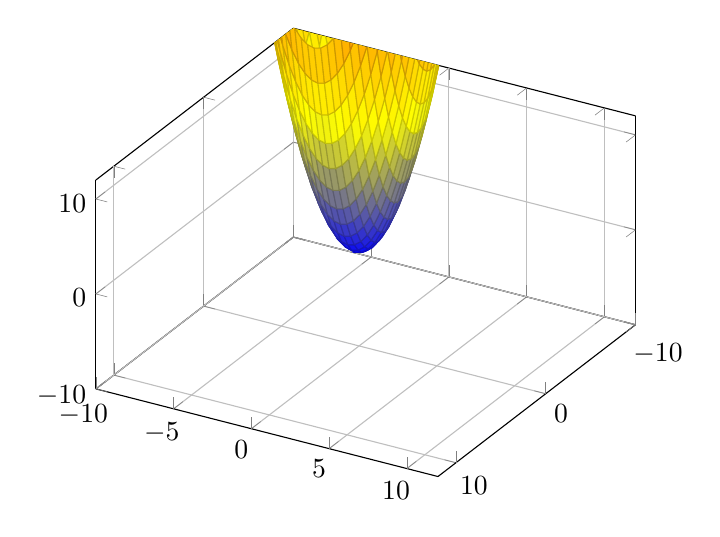
\begin{tikzpicture}
  \begin{axis}[
    view={120}{40},
    grid=major,
    xmin=-10,xmax=10,
    ymin=-10,ymax=10,
    zmin=-10,zmax=10,
    enlargelimits=upper,
    trig format plots=rad,
  ]
   \addplot3[surf] {x^2+y^2};
  \end{axis}
\end{tikzpicture}



\end{document}